\section{Rectificadores}
\label{sec:rect}
\subsection{Rectificador de media onda simple}
\begin{figure}[H]
  \centering
      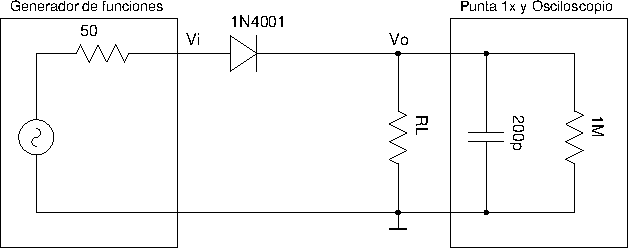
\includegraphics[width=0.8\textwidth]{gfxsantiago/FIG_CIRC_Rectificador_Simple_A.pdf}
  \caption{Circuito correspondiente al rectificador simple junto con el banco de medición utilizado y los equivalentes Thevenin de los instrumentos que fueron considerados para las simulaciones.}
  \label{fig:circ_3A}
\end{figure}
En esta parte del trabajo realizaremos mediciones relacionadas con el circuito que se muestra en la Figura \ref{fig:circ_3A}, el cual se denomina rectificador de media onda. El diodo utilizado es el 1N4001 y el resistor será de $R_{L} = 10 k\Omega$. El banco de medición correspondiente se muestra en la figura ya mencionada, el cual consta del circuito en cuestión excitado por una señal sinusoidal de $50Hz$ y amplitud $5V$ proveniente de un generador de funciones y los equivalentes de Thevenin correspondientes al generador de funciones y a la punta 1x que se conecta al osciloscopio.\\

\begin{figure}[H]
  \centering
      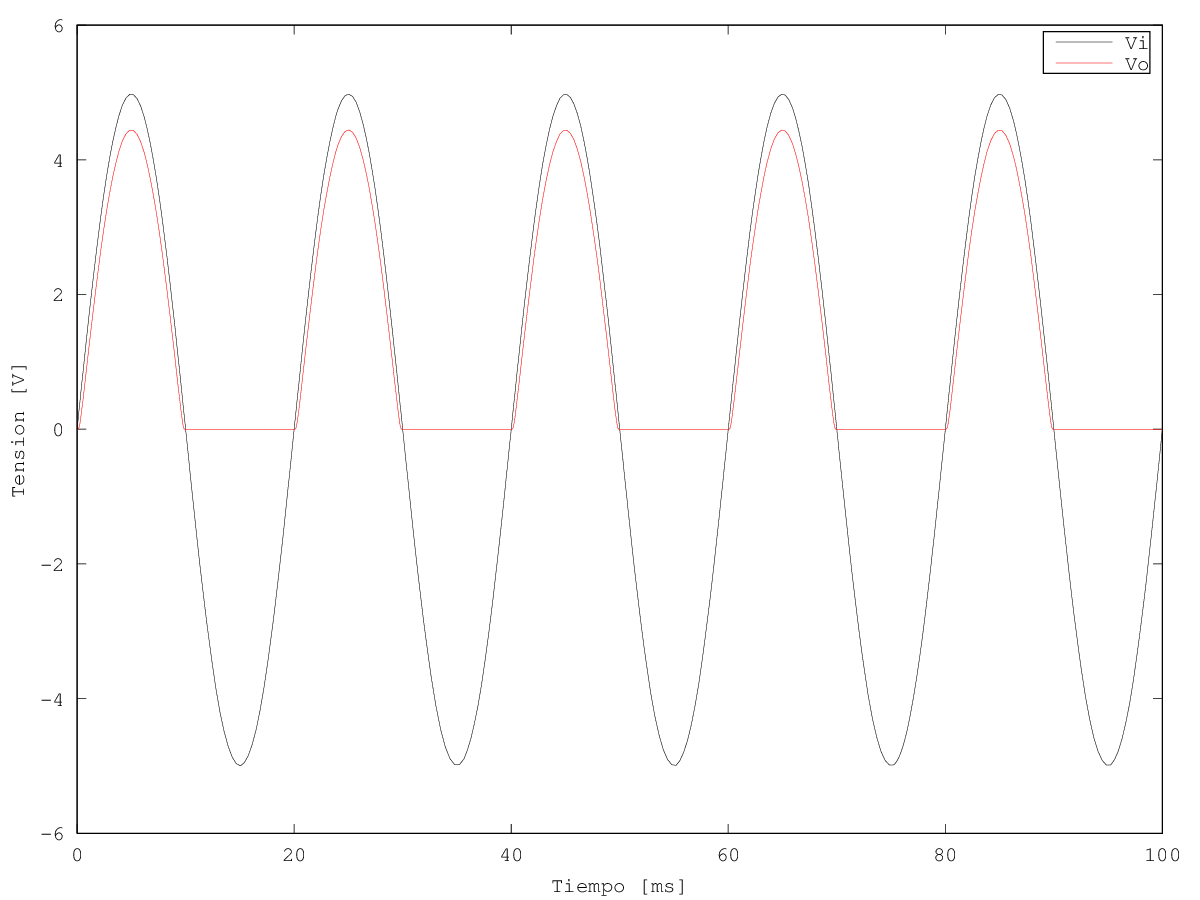
\includegraphics[width=0.8\textwidth]{gfxsantiago/FIG_SIM_Rectificador_Simple_3A1.png}
  \caption{Simulación de $v_{o}$ con señal de entrada de 50 Hz}
\end{figure}

\begin{figure}[H]
  \centering
      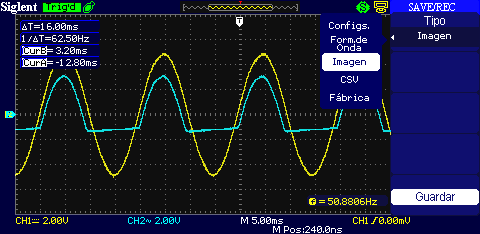
\includegraphics[width=0.8\textwidth]{gfxsantiago/FIG_MED_Rectificador_Simple_3A1.png}
  \caption{Medición de $v_{o}$ (azul) y $v_{i}$ (amarillo) con señal de entrada de 50 Hz}
\end{figure}

\noindent$\blacktriangle$\textbf{ ¿Por qué se utiliza una amplitud de 5 V en la excitación y no de 50 mV?}

La amplitud de la señal de excitación no puede ser de valores pequeños, como por ejemplo 50 mV, ya que en ese caso no se supera la tensión necesaria para que el diodo permita el paso de corriente.\\

A partir de las simulaciones realizadas se obtuvo un valor de 4,4 V pico para la tensión de salida $v_{o}$, cuyo valor medio (dado que se trata de una sinusoide rectificada) es $V_{o (medio)} = \hat{V}_{i}/\pi$ = 1,4 V.\\

\begin{figure}[H]
  \centering
      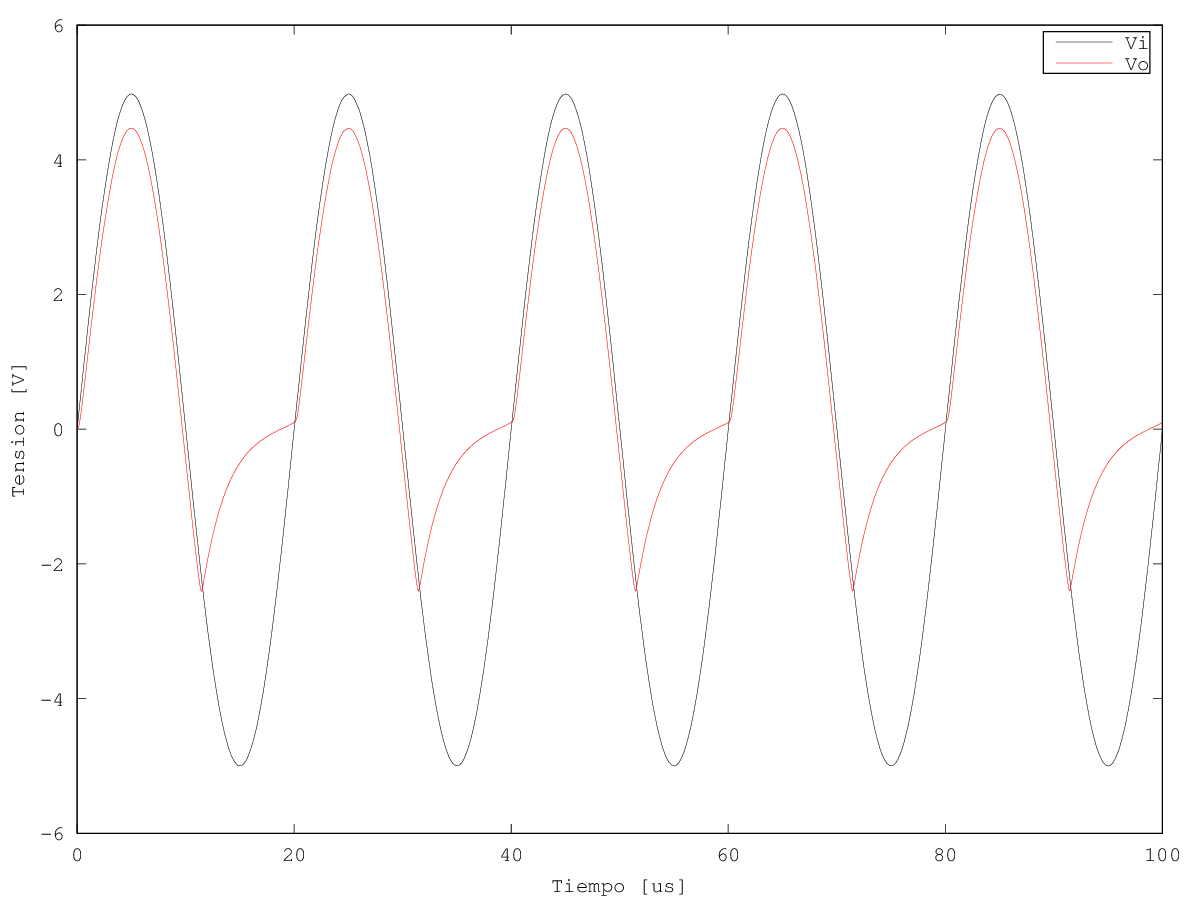
\includegraphics[width=0.8\textwidth]{gfxsantiago/FIG_SIM_Rectificador_Simple_3A2.png}
  \caption{Simulación de $v_{o}$ con señal de entrada de $50kHz$}
  \label{fig:sim_3A2}
\end{figure}

En estas mismas condiciones se incrementó la frecuencia de la señal de entrada a 50 kHz y la salida obtenida se puede observar en la Figura \ref{fig:sim_3A2}. En este caso, lo que sucede es que el tiempo de recuperación del diodo 1N4001 no permite la utilización de frecuencias tan altas, lo que tiene como consecuencia que no se puede utilizar el modelo de diodo al que estamos acostumbrados y eso se confirma al comparar las simulaciones para $v_{o}$ con $50Hz$ y $50kHz$.\\

Seguidamente se procede a conectar un capacitor de 47 $\mu F$ en paralelo a $R_{L}$, manteniendo el resto del banco de medición igual que antes (Figura \ref{fig:circ_3B}). Aquí, a partir de los datos obtenidos en las simulaciones y en las mediciones realizadas en el laboratorio es posible obtener valores de $v_{o (medio)}$, $v_{ripple}$ y el $z\%$ o porcentaje de ripple con la ayuda de las siguientes ecuaciones:

\begin{equation}
v_{ripple (ef)} = ( V_{o1 (ef)}^{2} + V_{o2 (ef)}^{2} + \ldots )^{1/2}
\end{equation}

\begin{equation}
z\% = 100 \frac{v_{ripple (ef)}}{v_{o (medio)}} 
\end{equation}

Para poder obtener los valores de $V_{oj (ef)}$, los cuales corresponden a las j-ésimas componentes de Fourier de la onda $V_{o}$ se hizo uso de la función FFT del LTSpice y del osciloscopio.\\

Los resultados se expresan a continuación en la Tabla \ref{table:rect_simple} y también se grafican las curvas correspondientes a $v_{o}$ para cada valor de $R_{L}$ en las Figuras \ref{fig:sim_3B1} a \ref{fig:med_3B3}. La presencia del capacitor genera que $v_{o}$ se mantenga dentro de un rango de valores denominado $v_{ripple}$ en vez de ser igual a la sinusoide rectificada como venia sucediendo. Si bien antes también podíamos considerar que había un capacitor en paralelo a la carga a partir del modelo de Thevenin de la punta 1x, este es de un valor muy pequeño como para que se acumule la carga necesaria para formar un ripple. Otra forma de ver esto último es a través de la constante de tiempo ($\tau$) del circuito que se forma, a partir del cual se puede aproximar el tiempo de carga y descarga del capacitor como:

\begin{equation}
5 \tau = 5 R C = 5 \cdot 10 k\Omega \cdot 200 pF = 10 \mu s
\end{equation}
mientras que al agregar el capacitor en paralelo, se modifica la constante de la siguiente manera: 

\begin{equation}
5 \tau = 5 R C = 5 \cdot 10 k\Omega \cdot 47\mu F = 2,35 s
\end{equation}

Además, al aumentar el valor de $R_{L}$ disminuye la corriente que puede circular por ella, con lo cual el capacitor se descarga más lentamente y $v_{ripple}$ disminuye.

Una de las observaciones que se pueden realizar sobre las gráficas realizadas es que al disminuir el valor de $R_{L}$, el semiciclo de la señal de entrada se deforma (esto es más claro en las figuras correspondientes a una carga de 1 $k\Omega$). Esto sucede porque el generador de funciones no es capaz de proveer la corriente que le esta demandando el circuito (la resistencia equivalente del generador tiene una caída de tensión interna) y solo tiene lugar en el semiciclo positivo ya que en el negativo el diodo no permite que circule corriente.

\begin{figure}[H]
  \centering
      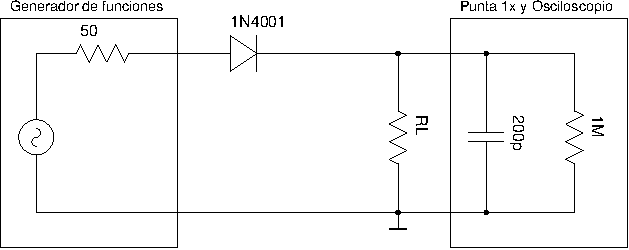
\includegraphics[width=0.8\textwidth]{gfxsantiago/FIG_CIRC_Rectificador_Simple_B.pdf}
  \caption{Circuito correspondiente al rectificador simple y capacitor junto con el banco de medición utilizado y los equivalentes Thevenin de los instrumentos que fueron considerados para las simulaciones.}
  \label{fig:circ_3B}
\end{figure}

\begin{figure}[H]
  \centering
      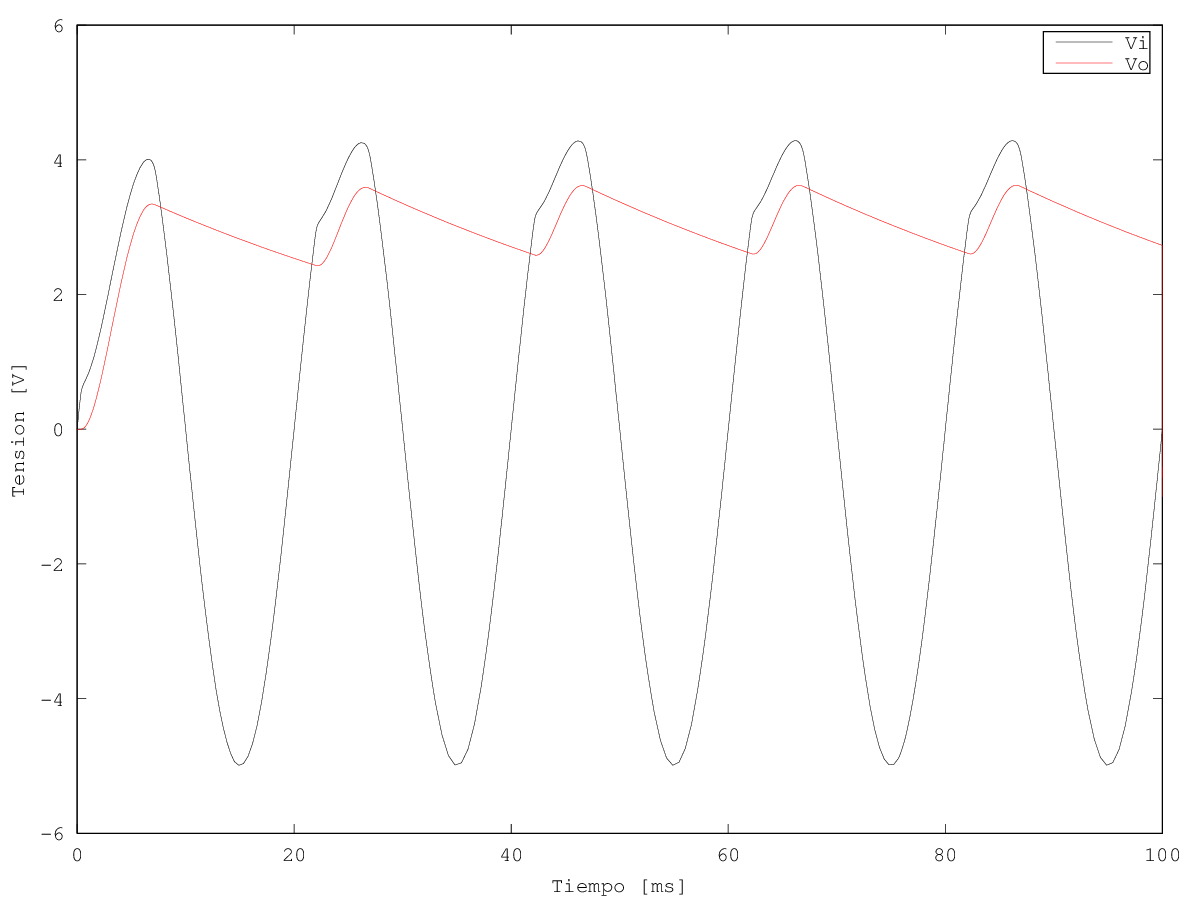
\includegraphics[width=0.8\textwidth]{gfxsantiago/FIG_SIM_Rectificador_Simple_3B1.png}
  \caption{Simulación de $v_{o}$ con $R_{L}$ = 1 $k\Omega$}
  \label{fig:sim_3B1}
\end{figure}

\begin{figure}[H]
  \centering
      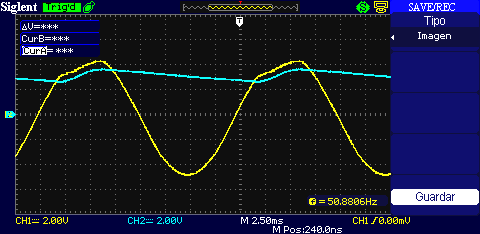
\includegraphics[width=0.8\textwidth]{gfxsantiago/FIG_MED_Rectificador_Simple_3B1.png}
  \caption{Medición de $v_{o}$ (azul) y $v_{i}$ (amarillo) con $R_{L}$ = 1 $k\Omega$}
\end{figure}

\begin{figure}[H]
  \centering
      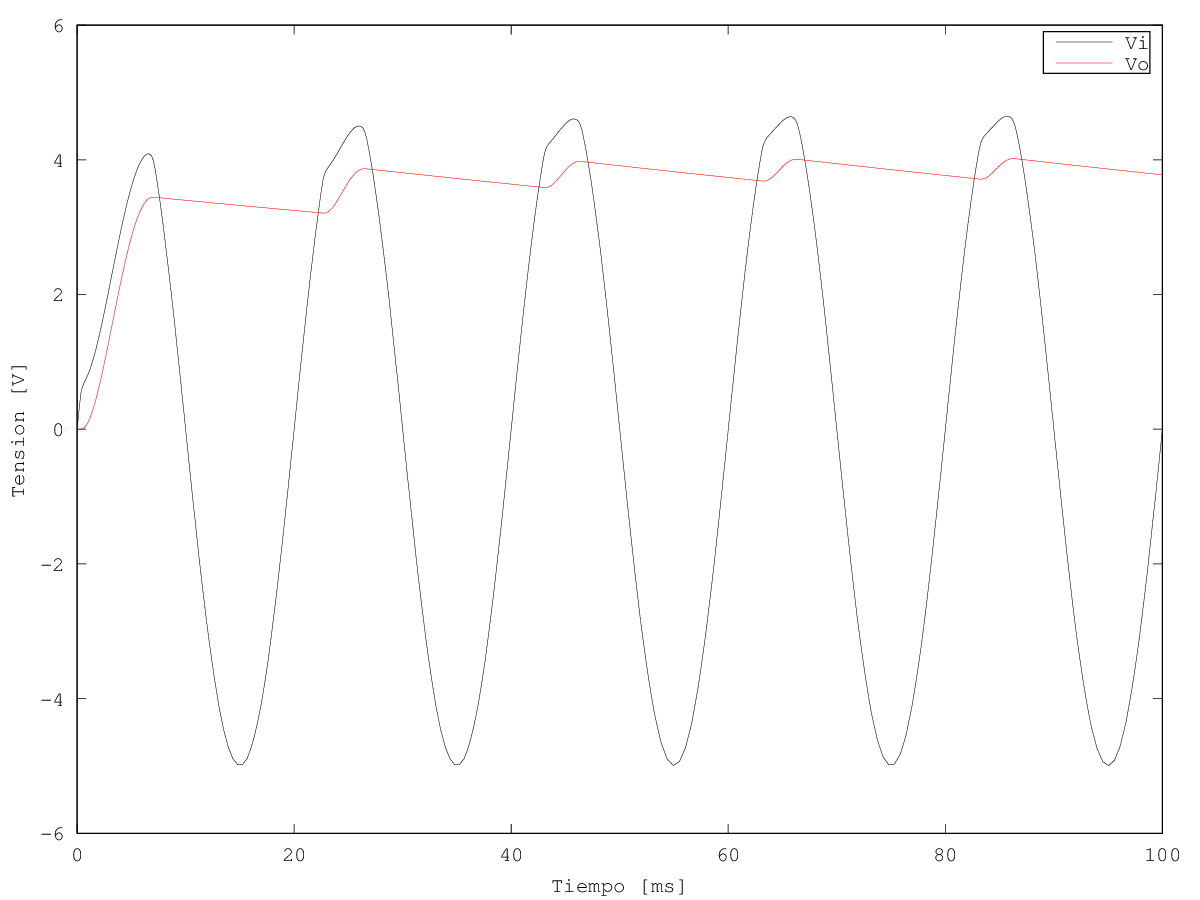
\includegraphics[width=0.8\textwidth]{gfxsantiago/FIG_SIM_Rectificador_Simple_3B2.png}
  \caption{Simulación de $v_{o}$ con $R_{L}$ = 4,7 $k\Omega$}
\end{figure}

\begin{figure}[H]
  \centering
      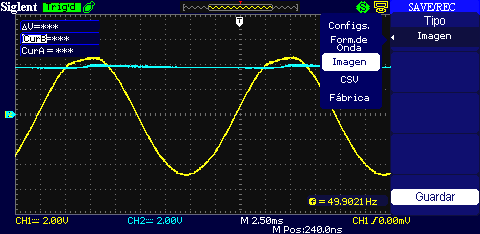
\includegraphics[width=0.8\textwidth]{gfxsantiago/FIG_MED_Rectificador_Simple_3B2.png}
  \caption{Medición de $v_{o}$ (azul) y $v_{i}$ (amarillo) con $R_{L}$ = 4,7 $k\Omega$}
\end{figure}

\begin{figure}[H]
  \centering
      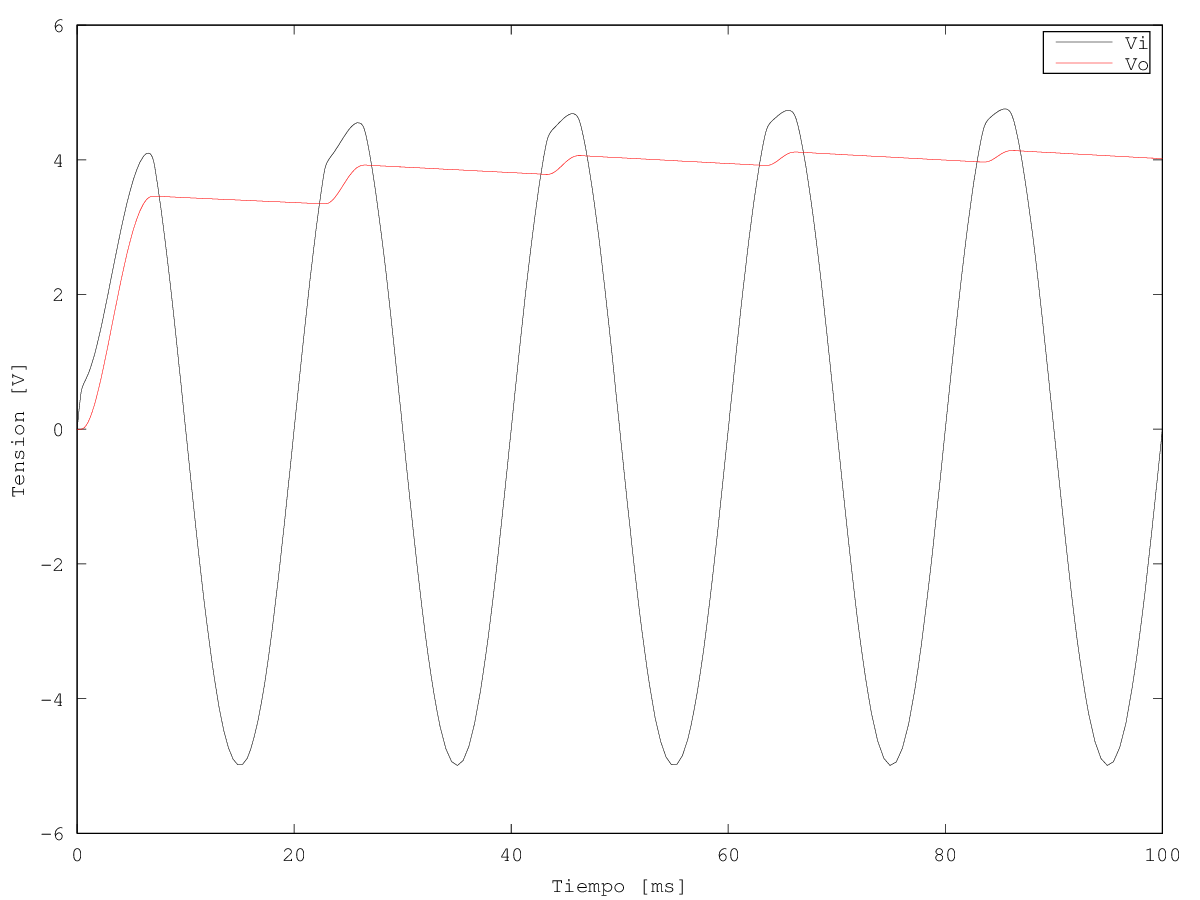
\includegraphics[width=0.8\textwidth]{gfxsantiago/FIG_SIM_Rectificador_Simple_3B3.png}
  \caption{Simulación de $v_{o}$ con $R_{L}$ = 10 $k\Omega$}
\end{figure}

\begin{figure}[H]
  \centering
      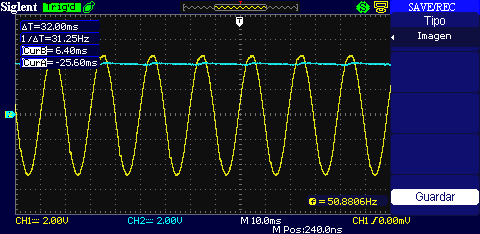
\includegraphics[width=0.8\textwidth]{gfxsantiago/FIG_MED_Rectificador_Simple_3B3.png}
  \caption{Medición de $v_{o}$ (azul) y $v_{i}$ (amarillo) con $R_{L}$ = 10 $k\Omega$}
  \label{fig:med_3B3}
\end{figure}

\begin{table}
\centering
\begin{tabular}{ccccccc}
\toprule
Carga $R_{L}$  & \multicolumn{3}{c}{Simulación}  & \multicolumn{3}{c}{Medición} \\

             & $v_{ripple(ef)}$    & $v_{o(medio)}$    &   $z\%$	& $v_{ripple(ef)}$    & $v_{o(medio)}$    &   $z\%$ \\
\midrule
1 $k\Omega$            & 0,33 V    & 3,68 V   & 9 \%	& 0,32 V    & 3,07 V   & 10\% \\
4,7 $k\Omega$            & 0,16 V    & 4,18 V   & 4 \%	& 0,08 V    & 3,83 V   & 2\% \\
10 $k\Omega$            & 0,1 V    & 4,28 V   & 2,5 \%	& 0,04 V    & 4,02 V   & 1\% \\
\bottomrule
\end{tabular}
\caption{}
\label{table:rect_simple}
\end{table}

\noindent$\blacktriangle$\textbf{ ¿Para qué sirve la curva llamada característica de regulación?}

A partir del análisis de la gráfica de dicha curva es posible analizar como varía la tensión media de salida del circuito según varía la carga $R_{L}$. Al aumentar la carga esto provoca una disminución de la corriente que circula por ella cuando el capacitor se esta descargando, con lo cual el ripple va haciéndose más pequeño (y $v_{o (medio)}$ aumenta).

\begin{figure}[H]
  \centering
      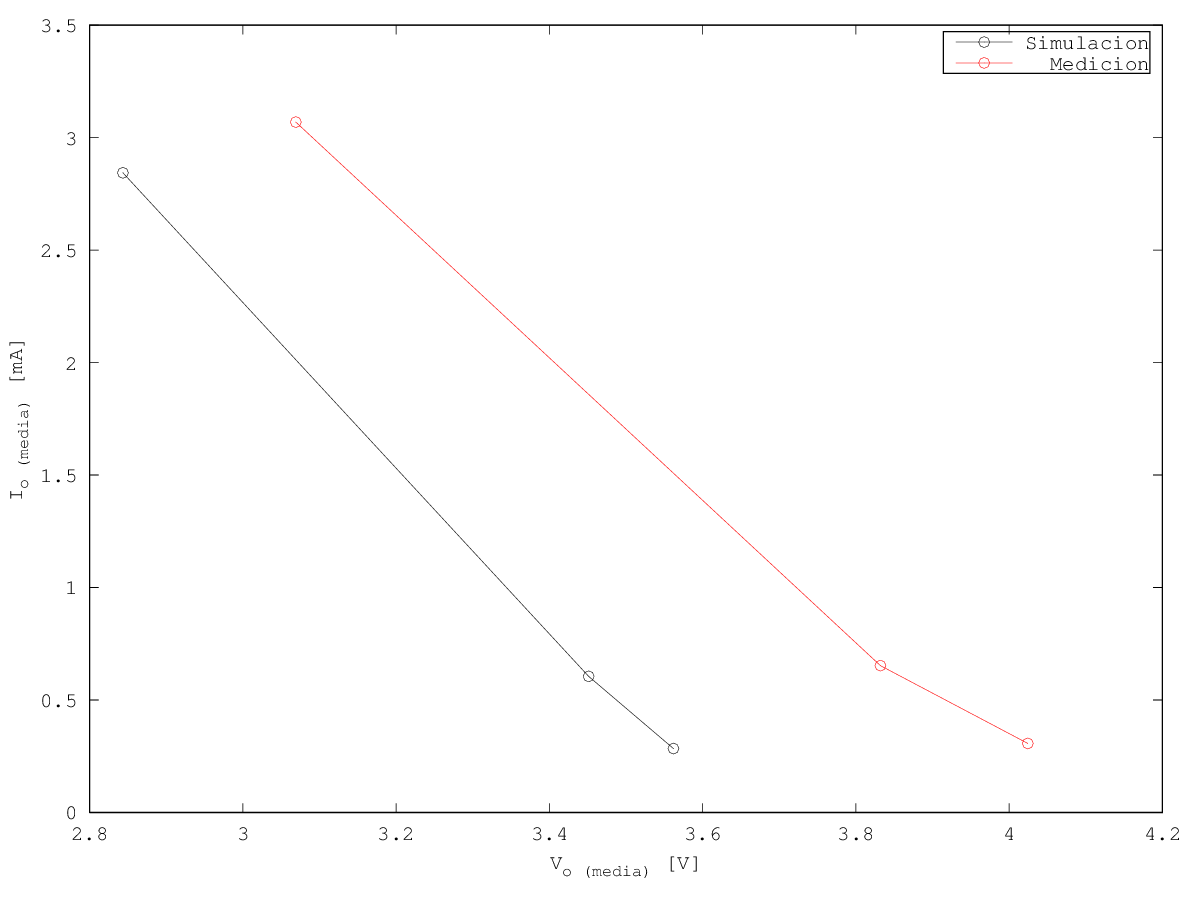
\includegraphics[width=0.8\textwidth]{gfxsantiago/FIG_Rectificador_Simple_Caracterisica_Regulacion.png}
  \caption{Curva característica de regulación obtenida en simulaciones y mediciones con osciloscopio.}
\end{figure}

\noindent$\blacktriangle$\textbf{ Proponer un banco de medición para medir la corriente a través del diodo. Justificar cualitativamente su forma y valores extremos.}

\begin{figure}[H]
  \centering
      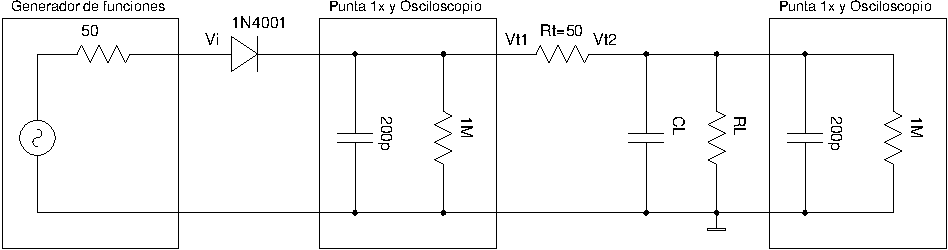
\includegraphics[width=0.8\textwidth]{gfxsantiago/FIG_CIRC_Rectificador_Simple_Corriente_Diodo.pdf}
  \caption{Circuito propuesto para la medición de la corriente que circula por el diodo.}
  \label{circ:corr_diodo}
\end{figure}

Una posibilidad es colocar una resistencia pequeña (en este caso se eligió utilizar una de 50 $\Omega$) a la que llamaremos $R_t$ en serie entre el diodo y la carga, como muestra la figura \ref{circ:corr_diodo}. En estas condiciones se puede medir la tensión que cae sobre dicho resistor colocando dos puntas de medición entre sus terminales, obteniendo finalmente la corriente que circula por el diodo haciendo:

\begin{equation}
i_D = i_{R_t} = \frac{v_{t2} - v_{t1}}{R_t}
\end{equation}

En la figura \ref{fig:sim_corr_diodo} se muestran los resultados de la simulación realizada utilizando el circuito propuesto, el cual coincide con lo esperado ya que el diodo solo conduce cuando la señal de entrada esta en el semiciclo positivo, generando una corriente en el sentido propuesto en la figura \ref{circ:corr_diodo}.

\begin{figure}[H]
  \centering
      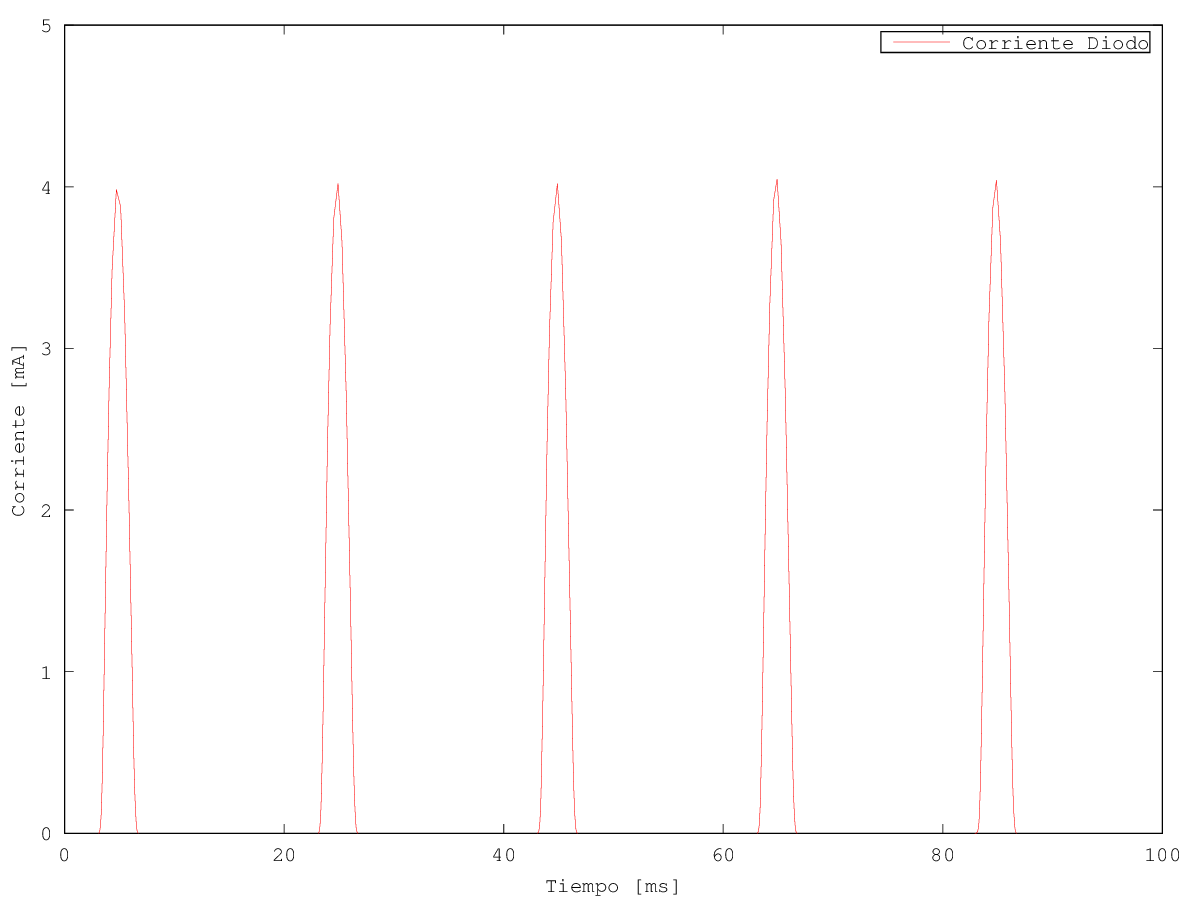
\includegraphics[width=0.8\textwidth]{gfxsantiago/FIG_SIM_Rectificador_Simple_Corriente_Diodo.png}
  \caption{Simulación de la corriente que circula por el diodo utilizando el método propuesto.}
  \label{fig:sim_corr_diodo}
\end{figure}

\noindent$\blacktriangle$\textbf{ Si en lugar de un rectificador de media onda se tuviese un puente rectificador de onda completa, ¿se esperaría un z\% mayor o menor?}

En el caso de un rectificador de onda completa, es fácil concluir que el porcentaje de rizado será menor que en el de media onda, ya que la tensión media de salida será mayor puesto que el tiempo durante el cual el capacitor se descarga es menor.\\


\subsection{Rectificador de media onda de precisión}
\begin{figure}[H]
  \centering
      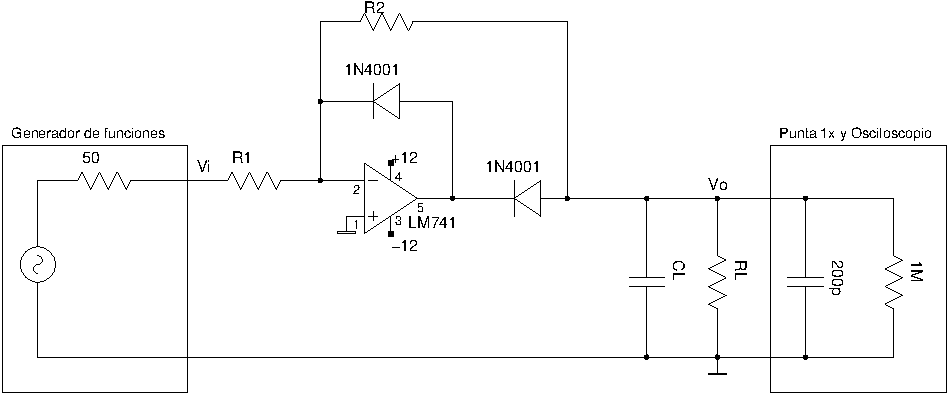
\includegraphics[width=0.8\textwidth]{gfxsantiago/FIG_CIRC_Rectificador_Precision_B.pdf}
  \caption{Circuito correspondiente al rectificador de precisión junto con el banco de medición utilizado y los equivalentes Thevenin de los instrumentos que fueron considerados para las simulaciones.}
  \label{fig:circ_4A}
\end{figure}
En este caso se utilizará un circuito cuya principal diferencia con respecto al del punto 3.1 es la presencia de un amplificador operacional. El circuito correspondiente se puede observar en la Figura \ref{fig:circ_4A}. Las mediciones a realizar son bajo las mismas condiciones que las del punto 3.1.\\

\begin{figure}[H]
  \centering
      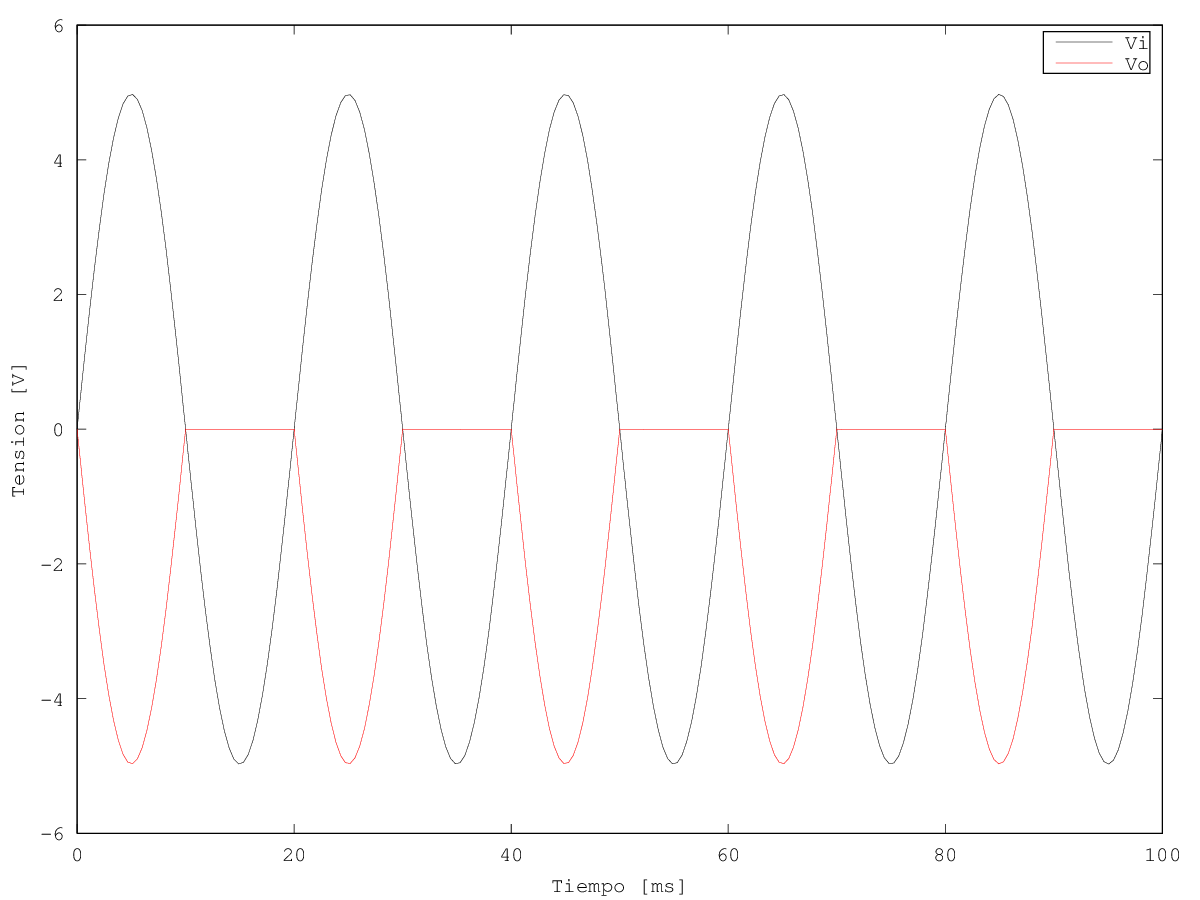
\includegraphics[width=0.8\textwidth]{gfxsantiago/FIG_SIM_Rectificador_Precision_4A1.png}
  \caption{Simulación de $v_{o}$ con señal de entrada de 50 Hz}
\end{figure}

\begin{figure}[H]
  \centering
      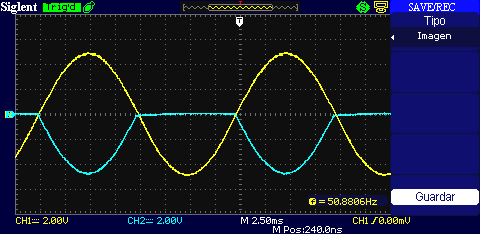
\includegraphics[width=0.8\textwidth]{gfxsantiago/FIG_MED_Rectificador_Precision_4A1.png}
  \caption{Medición de $v_{o}$ (Canal 2) y $v_{i}$ (Canal 1) con señal de entrada de $50Hz$}
\end{figure}

\begin{figure}[H]
  \centering
      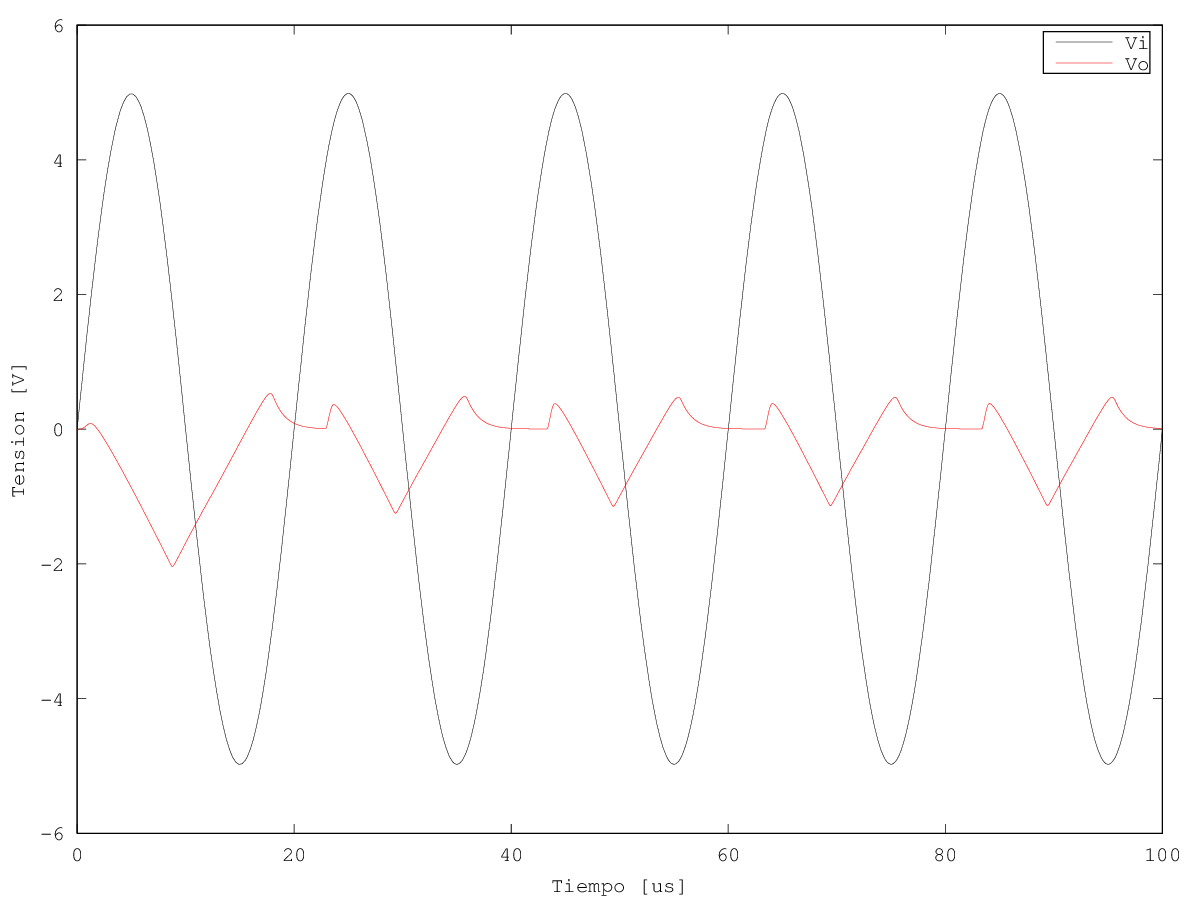
\includegraphics[width=0.8\textwidth]{gfxsantiago/FIG_SIM_Rectificador_Precision_4A2.png}
  \caption{Simulación de $v_{o}$ con señal de entrada de $50kHz$}
\end{figure}
En principio se utilizó como señal de entrada una sinusoide de 5 V pico y $50Hz$, junto con una resistencia de carga de 10 $k\Omega$. Es inmediato que el circuito, tal y como describe su nombre, rectifica manteniendo el semieje positivo de la señal de entrada prácticamente igual, a diferencia del caso del rectificador de media onda simple, en el cual había una diferencia entre $v_{o}$ y $v_{i}$ provocada por una caída de tensión en el diodo. Posteriormente se realizó la simulación correspondiente al mismo banco de trabajo pero modificando la frecuencia a $50kHz$. Las diferencias que se obtienen al realizar las simulaciones según se modifica la frecuencia de trabajo son notables y tiene la misma explicación que en el punto 3.1 para el diodo, a lo que hay que sumarle las variaciones respecto al modelo ideal de amplificador operacional según se aumenta la frecuencia, tal y como expresa la hoja de datos del AO LM741 (entre las cuales se destacan el aumento de la resistencia de salida, la disminución de la resistencia de entrada, etc.).

El funcionamiento del rectificador de precisión se puede subdividir según el semiciclo de la señal de entrada:
\begin{itemize}
  \item Semiciclo positivo: Viendo únicamente a las resistencias y considerando al amplificador como ideal es fácil concluir que $v_{o}$ será igual a $v_{i}$ pero de signo opuesto ya que la corriente que circula por ellas es la misma y son de igual valor (10 $k\Omega$). En este caso el diodo conectado entre la salida del operacional y $v_{o}$ conduce y genera una tensión de $v_{o} - 0,7 V$ en la salida del amplificador operacional, pero el diodo restante no permite que circule corriente puesto que no se cumple que $V_{D} < 0,7 V$, considerando a $V_{D}$ como la tensión entre el ánodo y cátodo del diodo.
  \item Semiciclo negativo: En este caso la corriente que circula por $R_{1}$ va en sentido contrario al de antes, por lo que el diodo que se encuentra entre la salida del operacional y el terminal de entrada negativo conduce esta corriente que esta provista por el AO. Dado que consideramos al operacional como ideal en ambos terminales de entrada hay una tierra virtual y como no circula corriente por $R_{2}$ se puede concluir que no cae tensión sobre ella y por lo tanto $v_{o} = 0 V$.
\end{itemize}

Luego, se procedió a colocar un capacitor de 47 $\mu F$ en paralelo a $R_{L}$, cuyo valor se fue aumentando al igual que en el punto anterior, es decir, 1 $k\Omega$, 4,7 $k\Omega$ y 10 $k\Omega$. Para estos tres casos se simuló y se midió con la ayuda de un osciloscopio el valor de $v_{o}$ y los resultados están expresados en las Figuras \ref{fig:sim_4B1} a \ref{fig:med_4B3}. Al igual que antes la presencia del capacitor genera que la tensión $v_{o}$ se mantenga dentro de un rango de valores reducido llamado $v_{ripple}$, y a medida que aumenta el valor de la resistencia $R_{L}$ el ripple va disminuyendo. Los resultados obtenidos para $v_{ripple(ef)}$, $v_{o(medio)}$ y $z\%$ correspondientes tanto a las simulaciones como a las mediciones se pueden observar en la tabla \ref{table:rect_precision}. \\

\begin{table}
\centering
\begin{tabular}{ccccccc}
\toprule
Carga $R_{L}$  & \multicolumn{3}{c}{Simulación}  & \multicolumn{3}{c}{Medición} \\

             & $v_{ripple(ef)}$    & $v_{o(medio)}$    &   $z\%$	& $v_{ripple(ef)}$    & $v_{o(medio)}$    &   $z\%$ \\
\midrule
1 $k\Omega$            & 0,3 V    & 4,15 V   & 7 \%	& 0,48 V    & 7,34 V   & 6\% \\
4,7 $k\Omega$            & 0,2 V    & 4,72 V   & 4 \%	& 0,16 V    & 8,40 V   & 2\% \\
10 $k\Omega$            & 0,17 V    & 4,8 V   & 3,5 \%	& 0,12 V    & 8,63 V   & 1\% \\
\bottomrule
\end{tabular}
\caption{}
\label{table:rect_precision}
\end{table}

\begin{figure}[H]
  \centering
      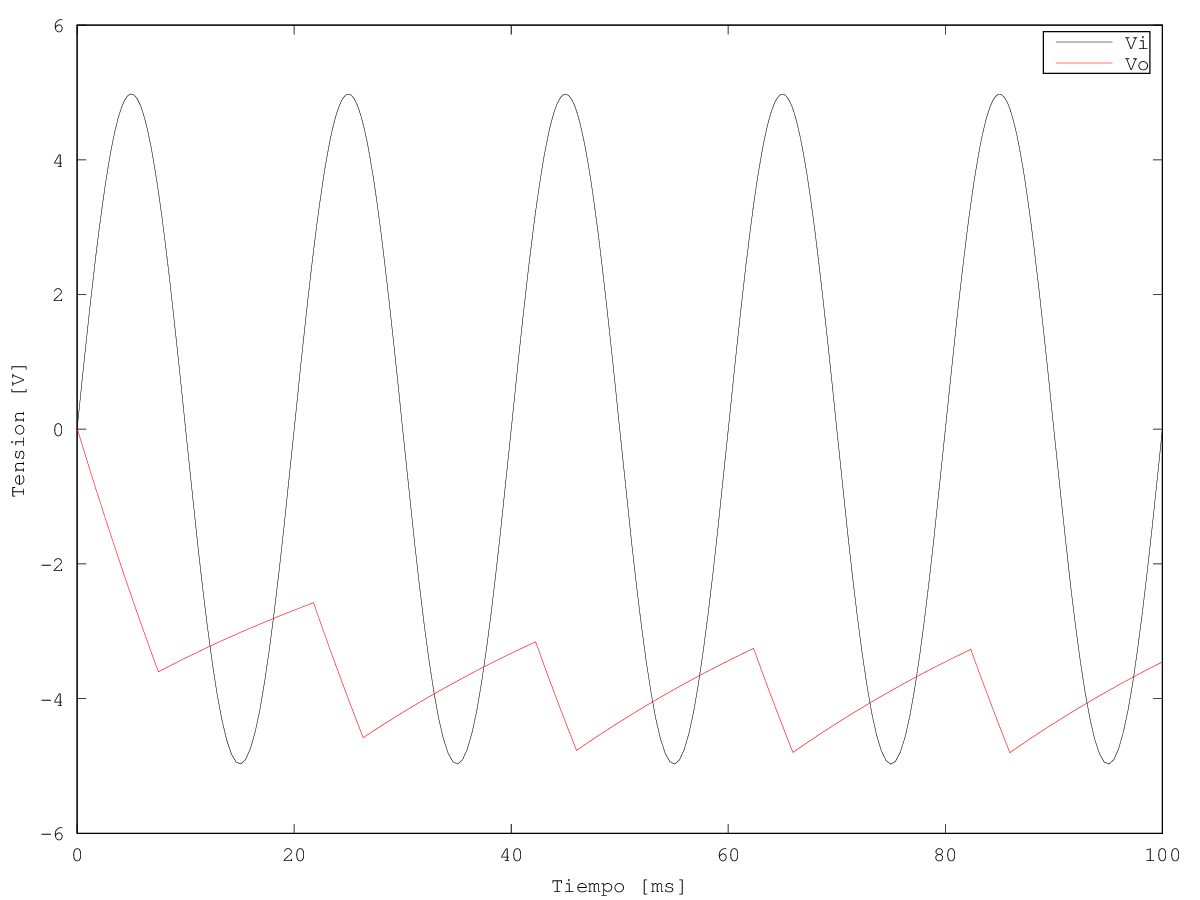
\includegraphics[width=0.8\textwidth]{gfxsantiago/FIG_SIM_Rectificador_Precision_4B1.png}
  \caption{Simulación de $v_{o}$ con $R_{L}$ = 1 $k\Omega$}
  \label{fig:sim_4B1}
\end{figure}

\begin{figure}[H]
  \centering
      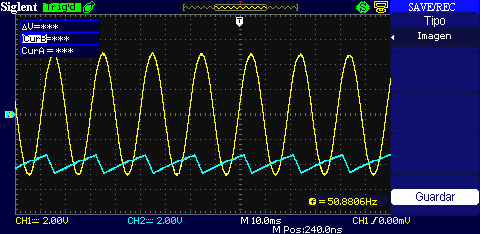
\includegraphics[width=0.8\textwidth]{gfxsantiago/FIG_MED_Rectificador_Precision_4B1.png}
  \caption{Medición de $v_{o}$ (Canal 2) y $v_{i}$ (Canal 1) con $R_{L}$ = 1 $k\Omega$}
\end{figure}

\begin{figure}[H]
  \centering
      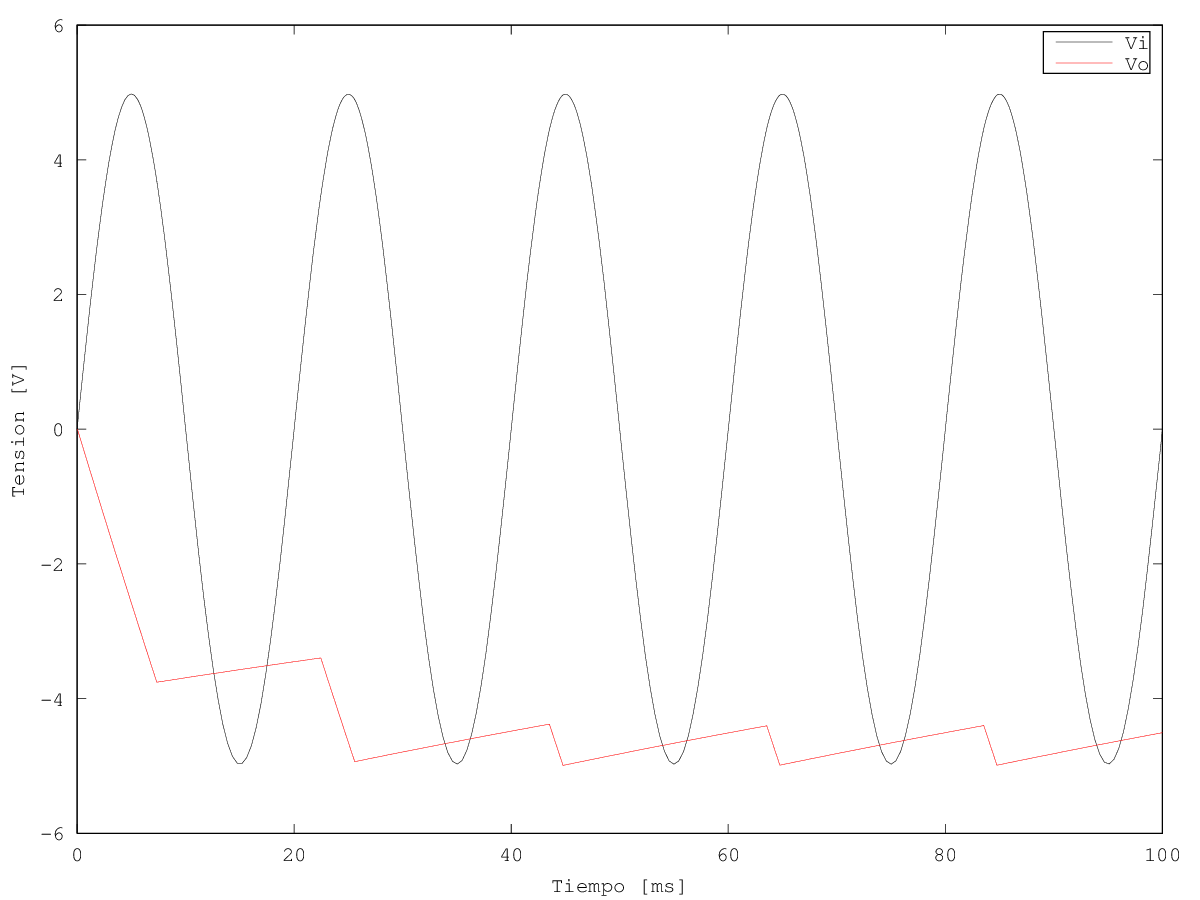
\includegraphics[width=0.8\textwidth]{gfxsantiago/FIG_SIM_Rectificador_Precision_4B2.png}
  \caption{Simulación de $v_{o}$ con $R_{L}$ = 4,7 $k\Omega$}
\end{figure}

\begin{figure}[H]
  \centering
      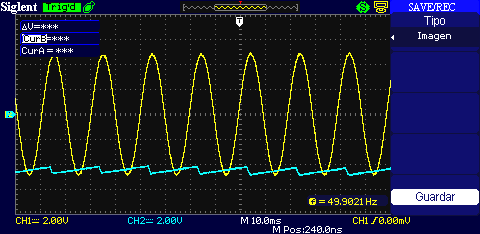
\includegraphics[width=0.8\textwidth]{gfxsantiago/FIG_MED_Rectificador_Precision_4B2.png}
  \caption{Medición de $v_{o}$ (Canal 2) y $v_{i}$ (Canal 1) con $R_{L}$ = 4,7 $k\Omega$}
\end{figure}

\begin{figure}[H]
  \centering
      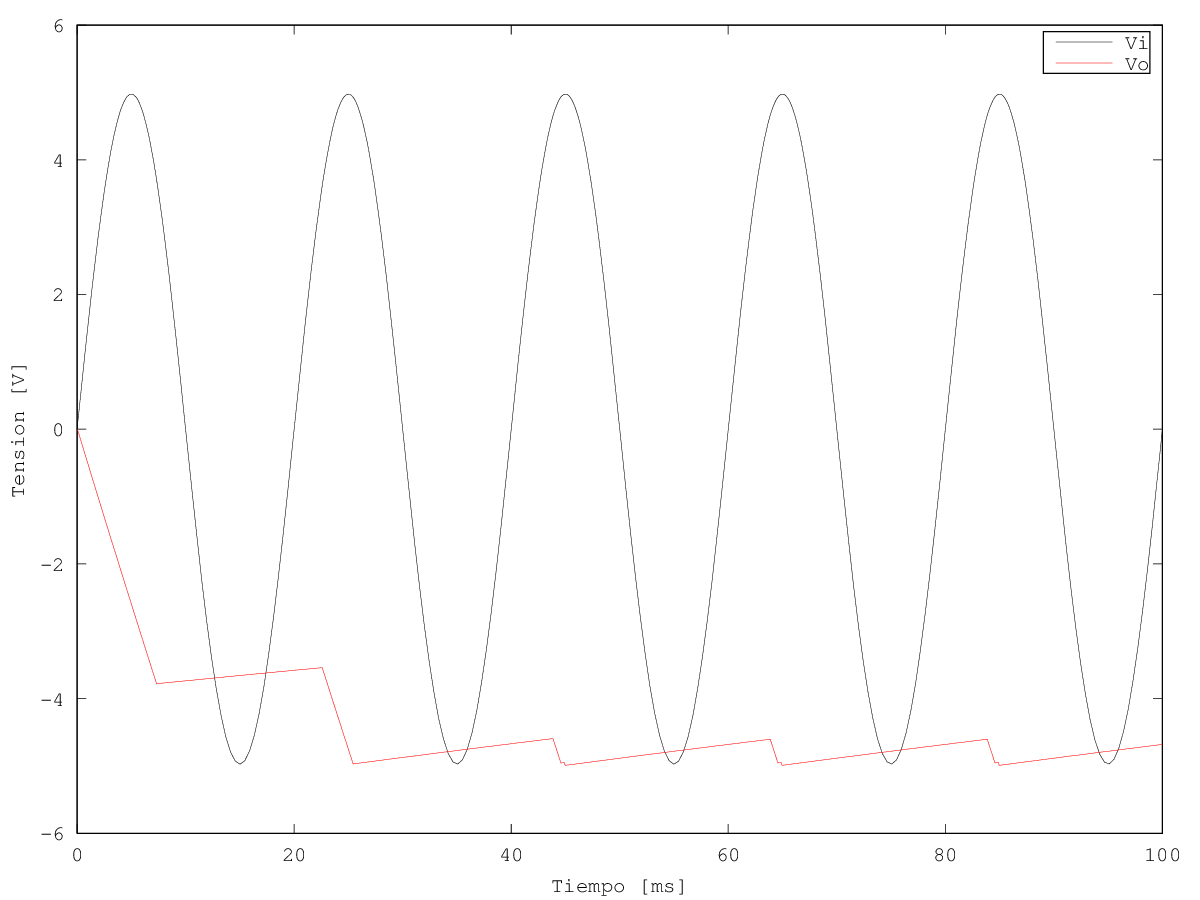
\includegraphics[width=0.8\textwidth]{gfxsantiago/FIG_SIM_Rectificador_Precision_4B3.png}
  \caption{Simulación de $v_{o}$ con $R_{L}$ = 10 $k\Omega$}
\end{figure}

\begin{figure}[H]
  \centering
      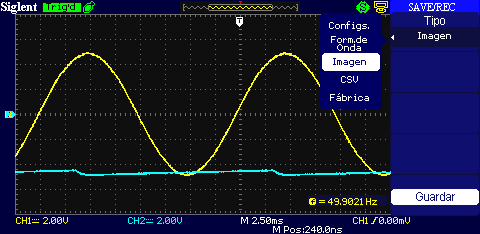
\includegraphics[width=0.8\textwidth]{gfxsantiago/FIG_MED_Rectificador_Precision_4B3.png}
  \caption{Medición de $v_{o}$ (Canal 2) y $v_{i}$ (Canal 1) con $R_{L}$ = 10 $k\Omega$}
  \label{fig:med_4B3}
\end{figure}

\begin{figure}[H]
  \centering
      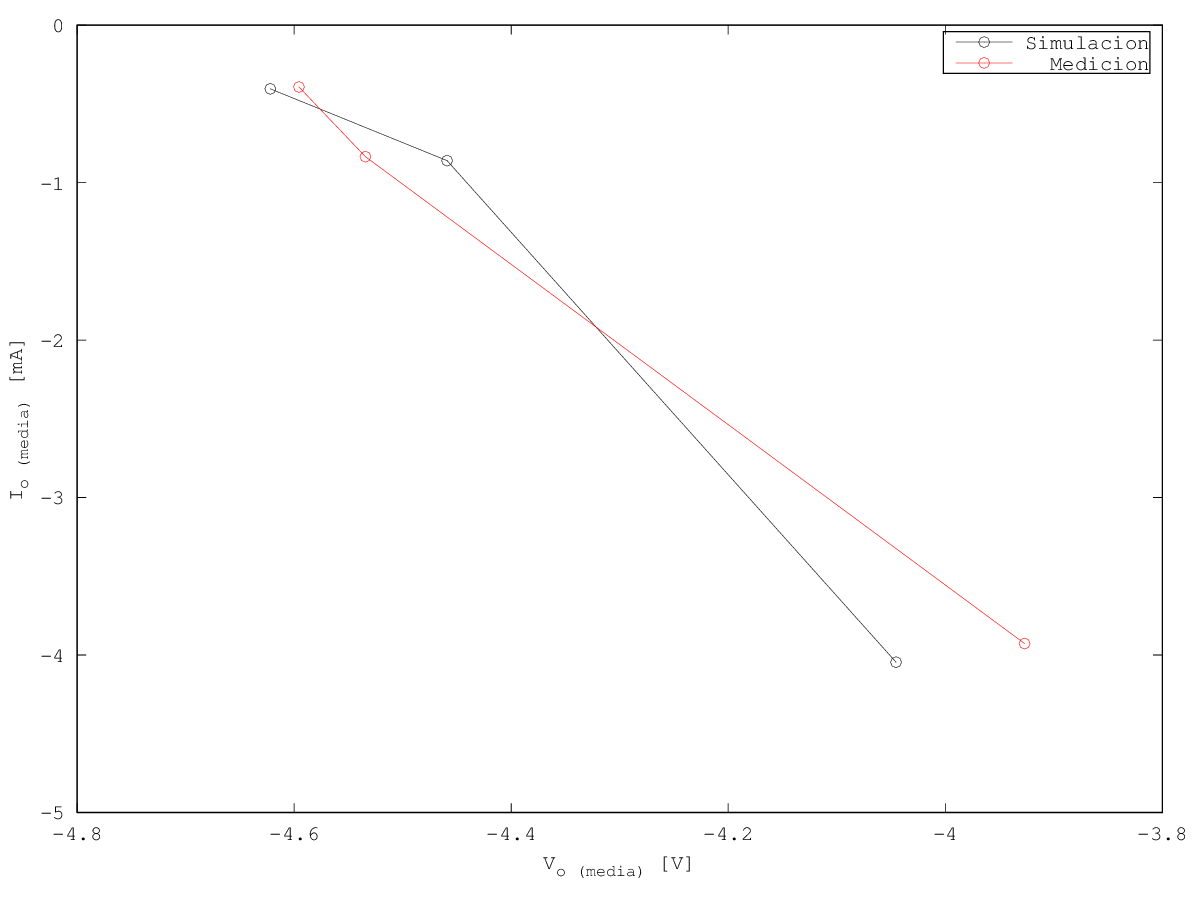
\includegraphics[width=0.8\textwidth]{gfxsantiago/FIG_Rectificador_Precision_Caracterisica_Regulacion.png}
  \caption{Curva característica de regulación obtenida en simulaciones y mediciones con osciloscopio.}
\end{figure}

\noindent$\blacktriangle$\textbf{ ¿Qué sucede si se reemplaza $R_2$ = 10 $k\Omega$ por un resistor de 22 $k\Omega$?}

En estas condiciones, a partir del análisis del circuito se puede predecir que el valor pico de $v_{o}$ aumentará prácticamente el doble. Esto se verifica tanto en las simulaciones (Figura \ref{fig:sim_4C}) y en las mediciones (Figura \ref{fig:med_4C}) pero también se observa que la señal tiene distorsión en los picos . Esto sucede debido a que en esos casos la tensión de salida es superior a lo que puede proveer el operacional.\\

\begin{figure}[H]
  \centering
      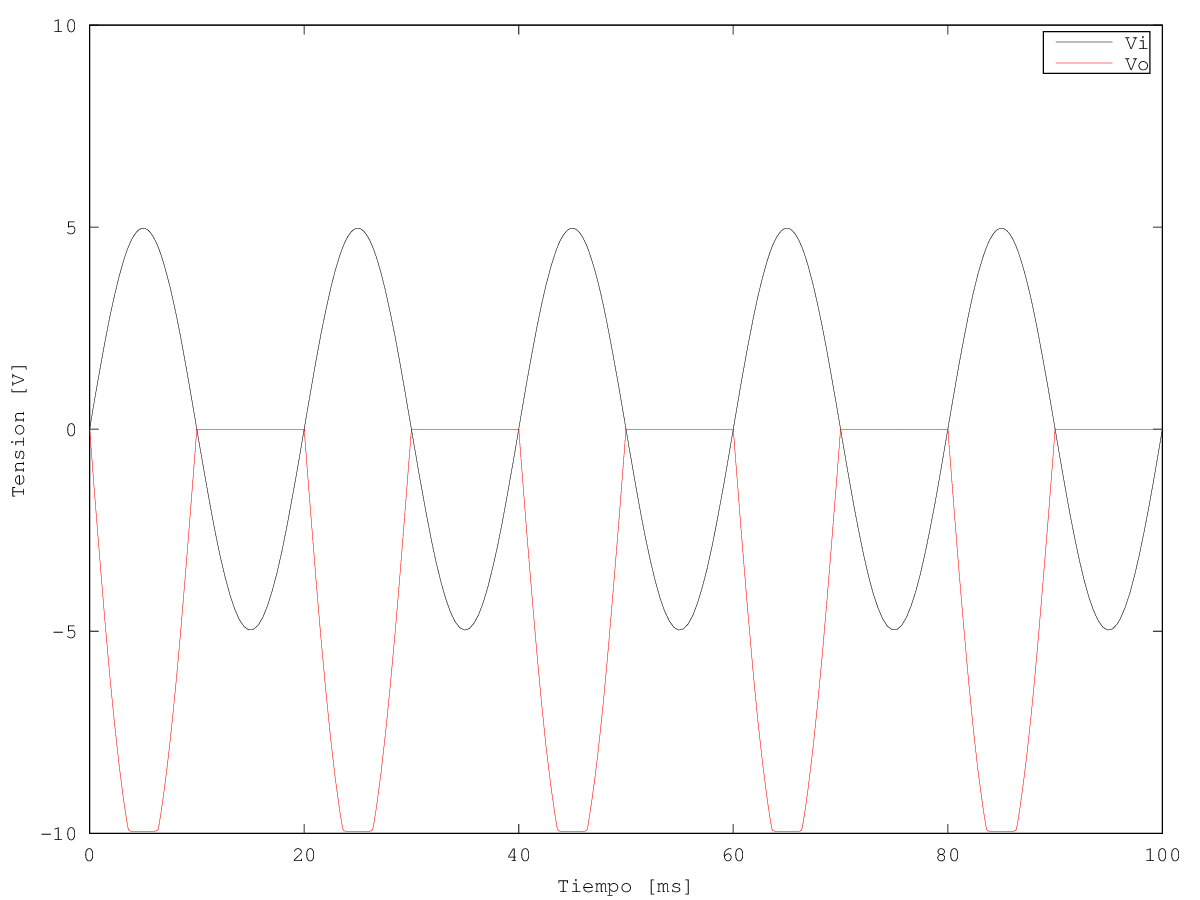
\includegraphics[width=0.8\textwidth]{gfxsantiago/FIG_SIM_Rectificador_Precision_4C.png}
  \caption{Simulación de $v_{o}$ con $R_{2}$ = 22 $k\Omega$}
  \label{fig:sim_4C}
\end{figure}

\begin{figure}[H]
  \centering
      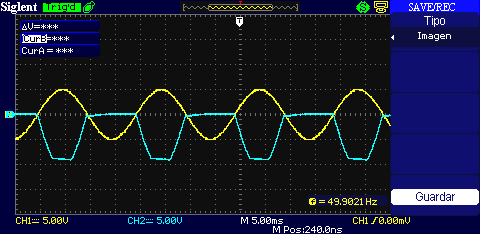
\includegraphics[width=0.8\textwidth]{gfxsantiago/FIG_MED_Rectificador_Precision_4C.png}
  \caption{Medición de $v_{o}$ (Canal 2) y $v_{i}$ (Canal 1) con $R_{2}$ = 22 $k\Omega$}
  \label{fig:med_4C}
\end{figure}

\noindent$\blacktriangle$\textbf{ ¿Qué sucede si se invierte la conexión de cada diodo?}

La inversión de las conexiones de cada diodo del circuito tendrá como consecuencia que cuando la señal de entrada se encuentra en su semiciclo positivo se tendrá 0 V en la salida mientras que cuando $v_{i}$ esta en el semiciclo negativo $v_{o}$ valdrá igual pero con signo opuesto. En la figura \ref{fig:sim_4D} se puede ver la gráfica de los datos obtenidos al simular esta situación, corroborando el análisis realizado.

\begin{figure}[H]
  \centering
      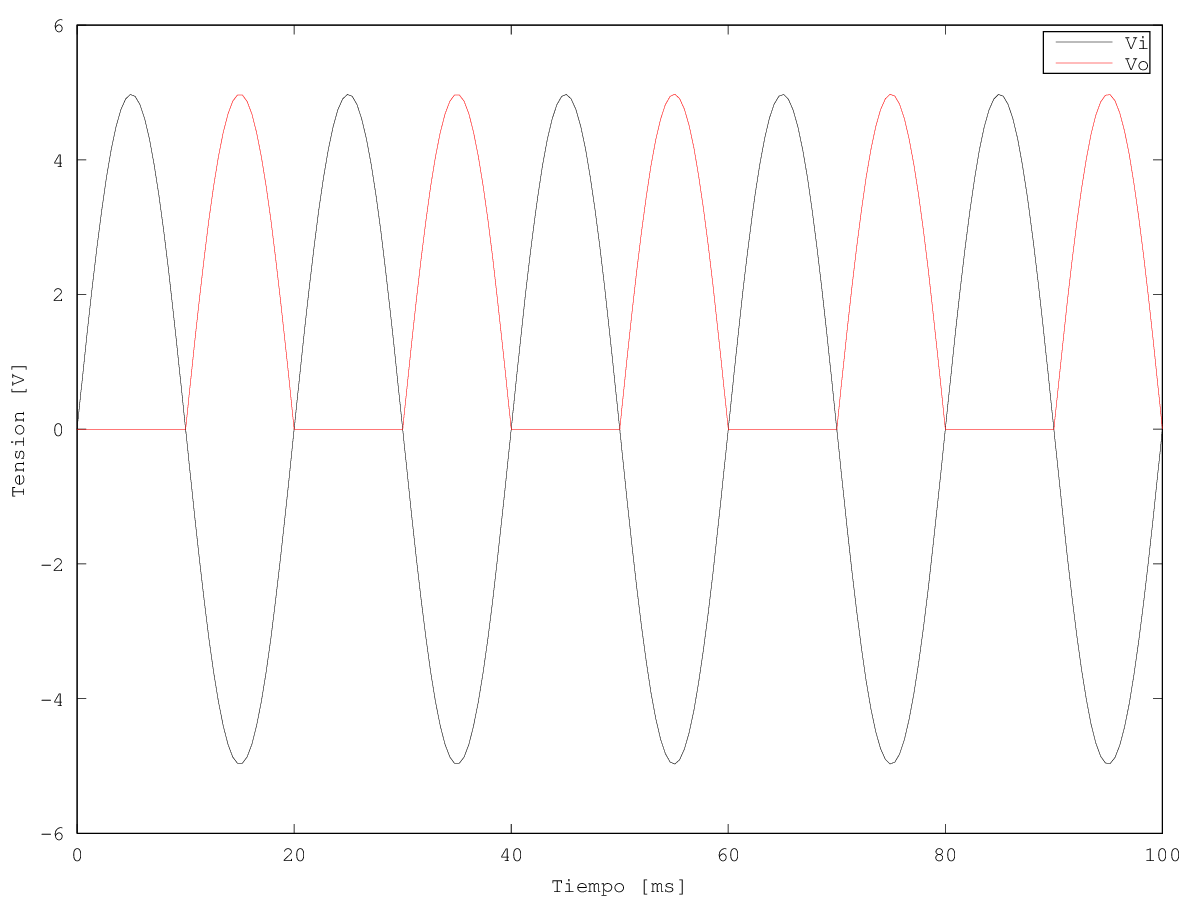
\includegraphics[width=0.8\textwidth]{gfxsantiago/FIG_SIM_Rectificador_Precision_4D.png}
  \caption{Simulación de $v_{o}$ con diodos invertidos}
  \label{fig:sim_4D}
\end{figure}
